
\section[Pacote 1]{Pacote 1}
No pacote de exercícios temos 2 módulos, o de classificação e o de resolução.

\subsection[Módulo 1]{Módulo 1}
O módulo de classificação objetiva fixar o reconhecimento e classificação de EDs. Este é composto de 6 fases: tipo, ordem, homogeneidade, linearidade, separável e exata respectivamente. Essas fases foram classificadas como sendo da mais fácil para a mais complexa. Para navegar entre as fases basta arrastar a tela para a direita.
Cada fase tem o domínio das suas perguntas e o número fixo de 20 equações que são selecionadas aleatoriamente de acordo com a fase.

As perguntas de tipo são: 
\begin{itemize}
	\item{}Escolha a ED ordinária
	\item{}Escolha a ED parcial
\end{itemize}


As perguntas de ordem são:
\begin{itemize}
	\item{}Escolha a ED de ordem 1
	\item{}Escolha a ED de ordem 2
	\item{}Escolha a ED de ordem 3
	\item{}Escolha a ED de ordem superior
\end{itemize}
 	

As perguntas de homogeneidade são:
\begin{itemize}
	\item{}Escolha a ED homogênea
	\item{}Escolha a ED NÃO homogênea
\end{itemize}
					
 
As perguntas de linearidade são:
\begin{itemize}
	\item{}Escolha a ED linear
	\item{}Escolha a ED NÃO linear
\end{itemize} 

As perguntas para a fase separável são:
\begin{itemize}
	\item{}Escolha a ED separável
	\item{}Escolha a ED NÃO separável
\end{itemize}

As perguntas se exata são:
\begin{itemize}
	\item{}Escolha a ED exata
	\item{}Escolha a ED NÃO exata
\end{itemize} 

\begin{figure}[H]
\centering
\caption{Tela inicial}
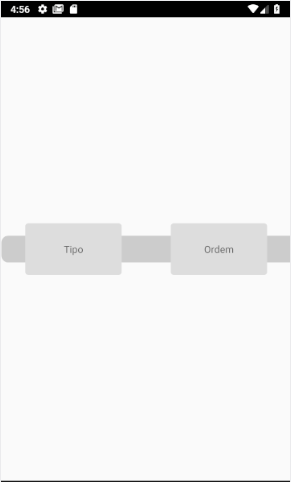
\includegraphics[scale=0.72]{figuras/modo_classificacao_1.png}
\small{Fonte: do próprio autor}
\end{figure}

\begin{figure}[H]
\centering
\caption{Tela inicial}
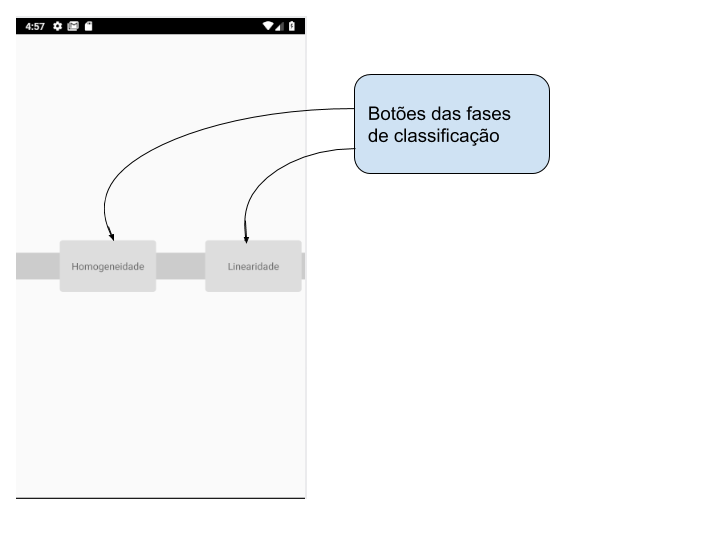
\includegraphics[scale=0.72]{figuras/modo_classificacao_2.png}
\small{Fonte: do próprio autor}
\end{figure}

\begin{figure}[H]
\centering
\caption{Tela inicial}
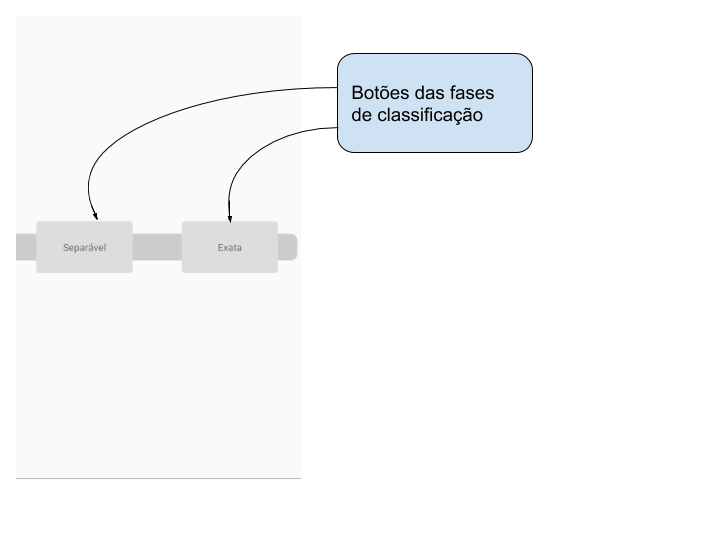
\includegraphics[scale=0.72]{figuras/modo_classificacao_3.png}
\small{Fonte: do próprio autor}
\end{figure}

As fases de classificação apresentam 4 equações como opção sendo que apenas 1 é a correta.
Ao pressionar cada opção por um tempo aparecerá a imagem da equação em uma janela modal para tentar melhorar a visualização.
Para escolher uma opção basta dar um toque na opção desejada.
Em caso de acerto da equação carregará automaticamente a próxima pergunta.
Em caso de erro aparecerá o \textit{feedback} da escolha da opção inválida.
Ao fim da fase será redirecionado novamente para o modo de classificação, após a parabenização do jogador, onde é possível escolher outra fase para jogar ou voltar para trocar o módulo.

\begin{figure}[H]
\centering
\caption{Tela inicial}
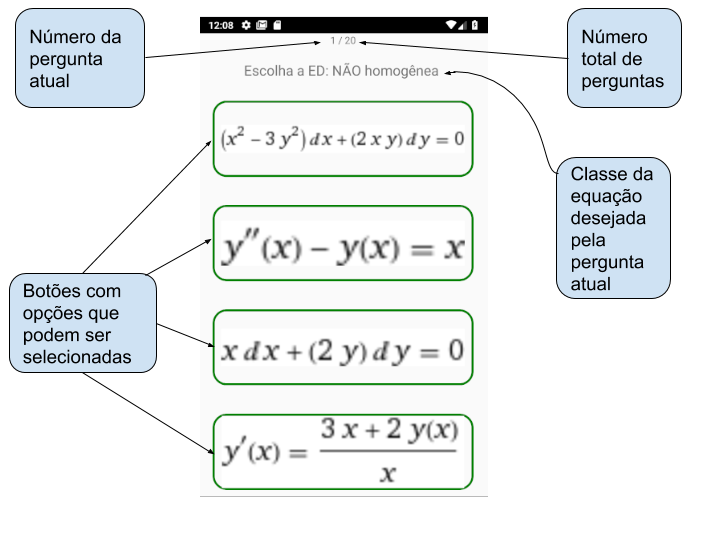
\includegraphics[scale=0.72]{figuras/ex_ed_n_homog.png}
\small{Fonte: do próprio autor}
\end{figure}

\begin{figure}[H]
\centering
\caption{Tela inicial}
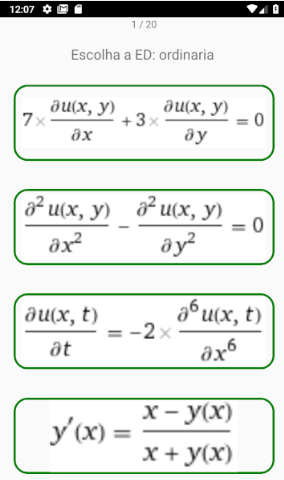
\includegraphics[scale=0.72]{figuras/ex_ed_ordinaria.png}
\small{Fonte: do próprio autor}
\end{figure}

\begin{figure}[H]
\centering
\caption{Tela inicial}
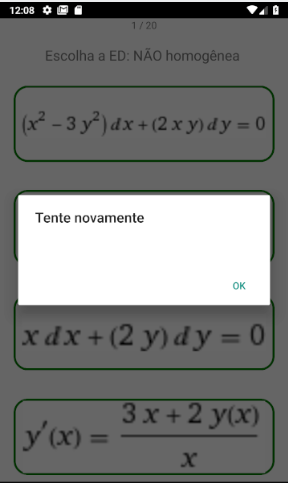
\includegraphics[scale=0.72]{figuras/tente_novamente.png}
\small{Fonte: do próprio autor}
\end{figure}

\begin{figure}[H]
\centering
\caption{Tela inicial}
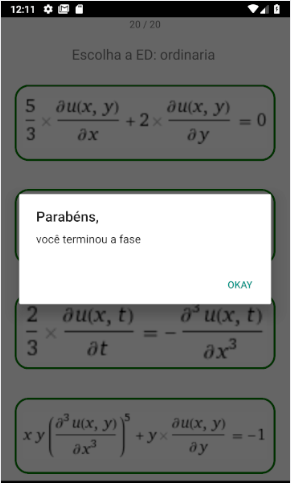
\includegraphics[scale=0.72]{figuras/fim_fase.png}
\small{Fonte: do próprio autor}
\end{figure}

\subsection[Módulo 2]{Módulo 2}

O módulo de resolução visa fixar o conhecimento de resolução de EDOs de 1ª e tem 4 fases. São elas homogênea, NÃO homogênea, exatas e NÃO exatas. Este módulo estão presentes APENAS equações diferenciais ordinárias de primeira ordem. 

\begin{figure}[H]
\centering
\caption{Tela inicial}
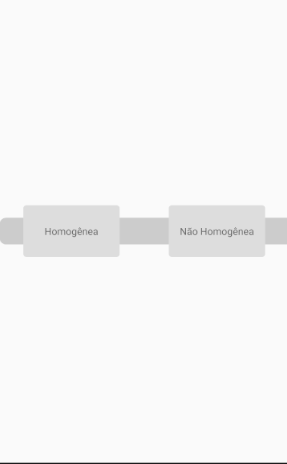
\includegraphics[scale=0.72]{figuras/modo_resolucao_1.png}
\small{Fonte: do próprio autor}
\end{figure}

\begin{figure}[H]
\centering
\caption{Tela inicial}
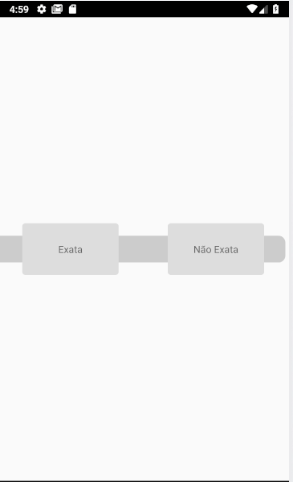
\includegraphics[scale=0.72]{figuras/modo_resolucao_2.png}
\small{Fonte: do próprio autor}
\end{figure}


Para isso jogaremos o jogo da memória, o qual tem o objetivo de encontrar as cartas gêmeas. Uma carta contém a EDO proposta e a carta gêmea contém a solução correta.

Existem 2 campos reservados na tela para mostrar as cartas selecionadas. O jogo é composto de 20 cartas, 10 EDO e 10 soluções de EDO. Cada carta é selecionada com um toque sobre ela, onde sua face será mostrada e seu conteúdo se mostrará em 1 dos 2 campos reservados. Cada clique inverte o lado da carta que está sendo mostrado. Ao selecionar 2 cartas haverá a comparação se são complementares (ou seja, pergunta e resposta). Em caso afirmativo, as cartas congelarão não sendo mais possível interagir com elas, em caso negativo apenas esconderão sua face para que inicie outra tentativa do jogador.

\begin{comment}
\subsection[Módulo 3]{Módulo 3}
– Jogo de classificação, perguntar técnica de resolução a ser utilizada em cada equação.

\end{comment}
